% =============================================================================
% HEXACORE — Presentación completa de la sustentación final
%
% Una sola presentación con las cuatro partes que pide el profesor, en su orden:
%   1. Cambios a la arquitectura: contenedores antiguo vs. nuevo (10 min)
%   2. Demostración del prototipo (10 min)
%   3. Asignación de cada atributo de calidad a cada integrante (1 diapositiva)
%   4. Diseño e implementación de los atributos (diapositivas y demostración en vivo)
%
% Se compila desde esta carpeta:  latexmk -pdf Sustentacion.tex
% Reutiliza las vistas de Diagrams/ y las láminas de Samuel
% (PresentacionAtributosSamuel.tex); el reparto está en DISTRIBUCION-ATRIBUTOS.md.
% =============================================================================
\documentclass[aspectratio=169,10pt,xcolor={table}]{beamer}

\usepackage[utf8]{inputenc}
\usepackage[T1]{fontenc}
\usepackage[spanish,es-noquoting,es-tabla]{babel}
\usepackage{booktabs}
\usepackage{array}
\usepackage{pifont}
\usepackage{pgfplots}
\usepackage{tikz}
\usepackage{xcolor}
\pgfplotsset{compat=1.18}
\usetikzlibrary{positioning, arrows.meta, shapes.geometric}

% --- Tema (el mismo de Presentacion.tex) ----------------------------------------
\usetheme{metropolis}
\metroset{block=fill, sectionpage=progressbar, numbering=fraction, progressbar=frametitle}

\definecolor{hexazul}{HTML}{1B3A5C}
\definecolor{hexaacento}{HTML}{0E7C7B}
\definecolor{hexaok}{HTML}{1B7F3B}
\definecolor{hexaparcial}{HTML}{B8860B}
\definecolor{hexapend}{HTML}{8B1A1A}
\definecolor{hexagris}{HTML}{F2F4F6}

\setbeamercolor{frametitle}{bg=hexazul, fg=white}
\setbeamercolor{progress bar}{fg=hexaacento, bg=hexagris}
\setbeamercolor{title separator}{fg=hexaacento}
\setbeamercolor{alerted text}{fg=hexaacento}
\setbeamercolor{block title}{bg=hexagris, fg=hexazul}
\setbeamercolor{block body}{bg=hexagris!45}

\newcommand{\ok}{\textcolor{hexaok}{\ding{51}}}
\newcommand{\parcial}{\textcolor{hexaparcial}{\ding{108}}}
\newcommand{\pend}{\textcolor{hexapend}{\ding{55}}}
\newcommand{\cifra}[1]{{\color{hexaacento}\textbf{#1}}}

\setbeamersize{text margin left=0.7cm, text margin right=0.7cm}
\renewcommand{\arraystretch}{1.08}
\newcolumntype{L}[1]{>{\raggedright\arraybackslash}p{#1}}
\newcolumntype{C}[1]{>{\centering\arraybackslash}p{#1}}

\newcommand{\codigo}[2]{\href{https://github.com/Emperador24/HEXACORE/blob/develop/#1}{#2}}
% Nota al pie de cada lámina: quién la presenta y de dónde sale la evidencia.
\newcommand{\nota}[1]{\par\smallskip{\scriptsize\color{hexaacento}#1}}
% Las láminas de Samuel traen la franja del guion de Presentacion.tex; aquí los
% tiempos los da la agenda, así que la franja no se muestra.
\newcommand{\franja}[1]{}
% Activa en PresentacionAtributosSamuel.tex las láminas de ZeroTier y de tiempo real.
\def\SustentacionCompleta{}

\title{Sistema Integral de Gestión de Eventos}
\subtitle{Sustentación final · arquitectura, prototipo y atributos de calidad}
\author{Daniel Cristancho · Samuel Emperador · Sebastián Sánchez · Diego Coronado}
\institute{Pontificia Universidad Javeriana · HEXACORE}
\date{Noviembre de 2026}

% Vistas vigentes (ADR-16), reutilizadas por SAD, C4, resumen, propuesta y presentación.
% Una sola fuente: las especificaciones de ../Archify/*.json. Cada macro incluye el PDF
% vectorial que exporta Archify (../ArchifyPDF), el mismo dibujo que el HTML interactivo.
% Para cambiar una vista: editar su JSON, regenerar HTML y PDF (ver ../Archify/README.md)
% y recompilar los documentos. Las rutas son relativas a Documentation/Work.
\providecommand{\HexVista}[1]{%
  \includegraphics[width=\textwidth,height=0.78\textheight,keepaspectratio]{Diagrams/ArchifyPDF/#1.pdf}}
\providecommand{\HexContexto}{\HexVista{01-contexto}}
\providecommand{\HexContenedores}{\HexVista{02-contenedores}}
\providecommand{\HexComponentesNucleo}{\HexVista{03-componentes-nucleo}}
\providecommand{\HexComponentesBoleteria}{\HexVista{04-componentes-boleteria}}
\providecommand{\HexPanorama}{\HexVista{05-panorama}}
\providecommand{\HexSecuencia}{\HexVista{06-secuencia}}
\providecommand{\HexDespliegue}{\HexVista{07-despliegue}}
\providecommand{\HexDespliegueZeroTier}{\HexVista{09-despliegue-zerotier}}

\begin{document}

\begin{frame}[plain,shrink=5]
\setbeamerfont{title}{size=\Large}
\setbeamerfont{subtitle}{size=\normalsize}
\setbeamerfont{author}{size=\footnotesize}
\titlepage
\end{frame}

% ---------------------------------------------------------------------------
\begin{frame}{Agenda · máximo una hora}
\small
\begin{tabular}{@{}rL{5.2cm}L{4.6cm}r@{}}
\toprule
& \textbf{Bloque} & \textbf{Qué se ve} & \textbf{Tiempo}\\
\midrule
1 & Cambios a la arquitectura & Contenedores antiguos vs. nuevos y por qué & 10 min\\
2 & Demostración del prototipo & Casos de uso de cada integrante, en vivo & 10 min\\
3 & Asignación de atributos & Una lámina: quién responde por qué & 1 min\\
4 & Diseño e implementación de atributos & Escenario, tácticas, evidencia y demo en vivo & 32 min\\
& Preguntas & & 7 min\\
\bottomrule
\end{tabular}

\vspace{0.8em}
\textbf{Mientras tanto, en otro computador:} el pipeline de despliegue de Diego corre desde el
inicio, porque tarda varios minutos (lo pidió el profesor).
\end{frame}

% =============================================================================
\section{Cambios a la arquitectura}
% =============================================================================

\begin{frame}{Por qué cambió la arquitectura (ADR-16)}
\begin{itemize}\setlength\itemsep{0.5em}
\item \textbf{El problema:} coordinar programas, versiones, llamadas y datos costaba más que la
separación que daban. Las diez aplicaciones que existían no coincidían con los catorce servicios
que proponía ADR-14.
\item \textbf{La decisión:} un solo workspace de backend con \cifra{tres ejecutables}: Núcleo,
Boletería y Trabajador. Cada dominio es un módulo con su propio esquema.
\item \textbf{Lo que se conservó:} el comportamiento de cada caso de uso, el API Gateway como única
entrada, la mensajería por RabbitMQ y el JWT RS256.
\item \textbf{Lo que se acepta a cambio:} un fallo de la base o un despliegue afecta a varios
módulos a la vez; se versionan juntos.
\end{itemize}
\nota{Detalle: SAD, ADR-16 y sección «Arquitectura vigente».}
\end{frame}

\begin{frame}{Contenedores: antes y ahora}
\begin{columns}[T,onlytextwidth]
\column{0.49\textwidth}\centering
\textbf{Antes: propuesta ADR-14/15}

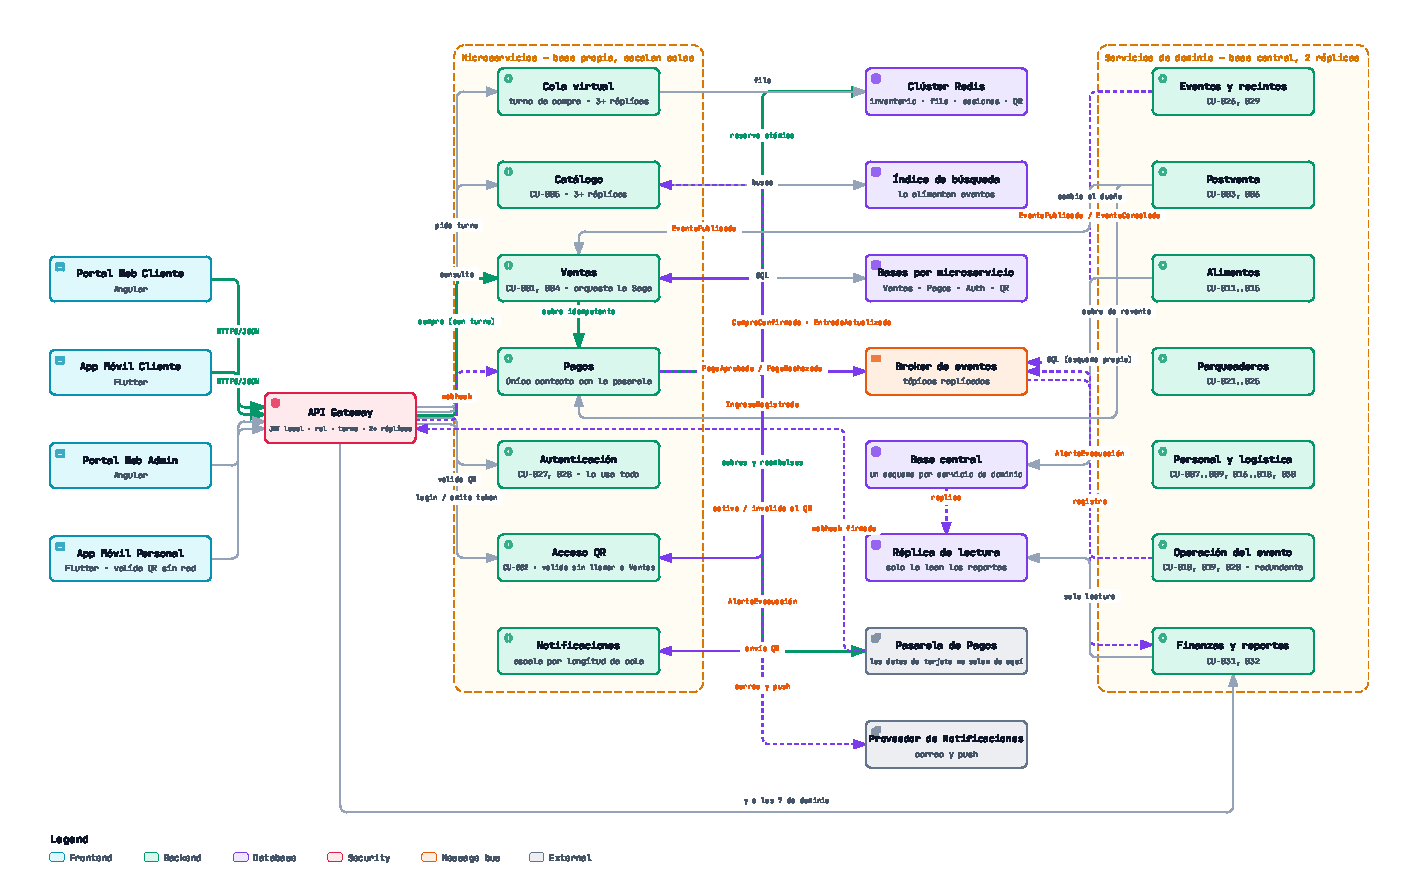
\includegraphics[width=\linewidth,height=0.6\textheight,keepaspectratio]{Historico/Contenedores-ADR14-15.pdf}
\column{0.49\textwidth}\centering
\textbf{Ahora: implementación ADR-16}

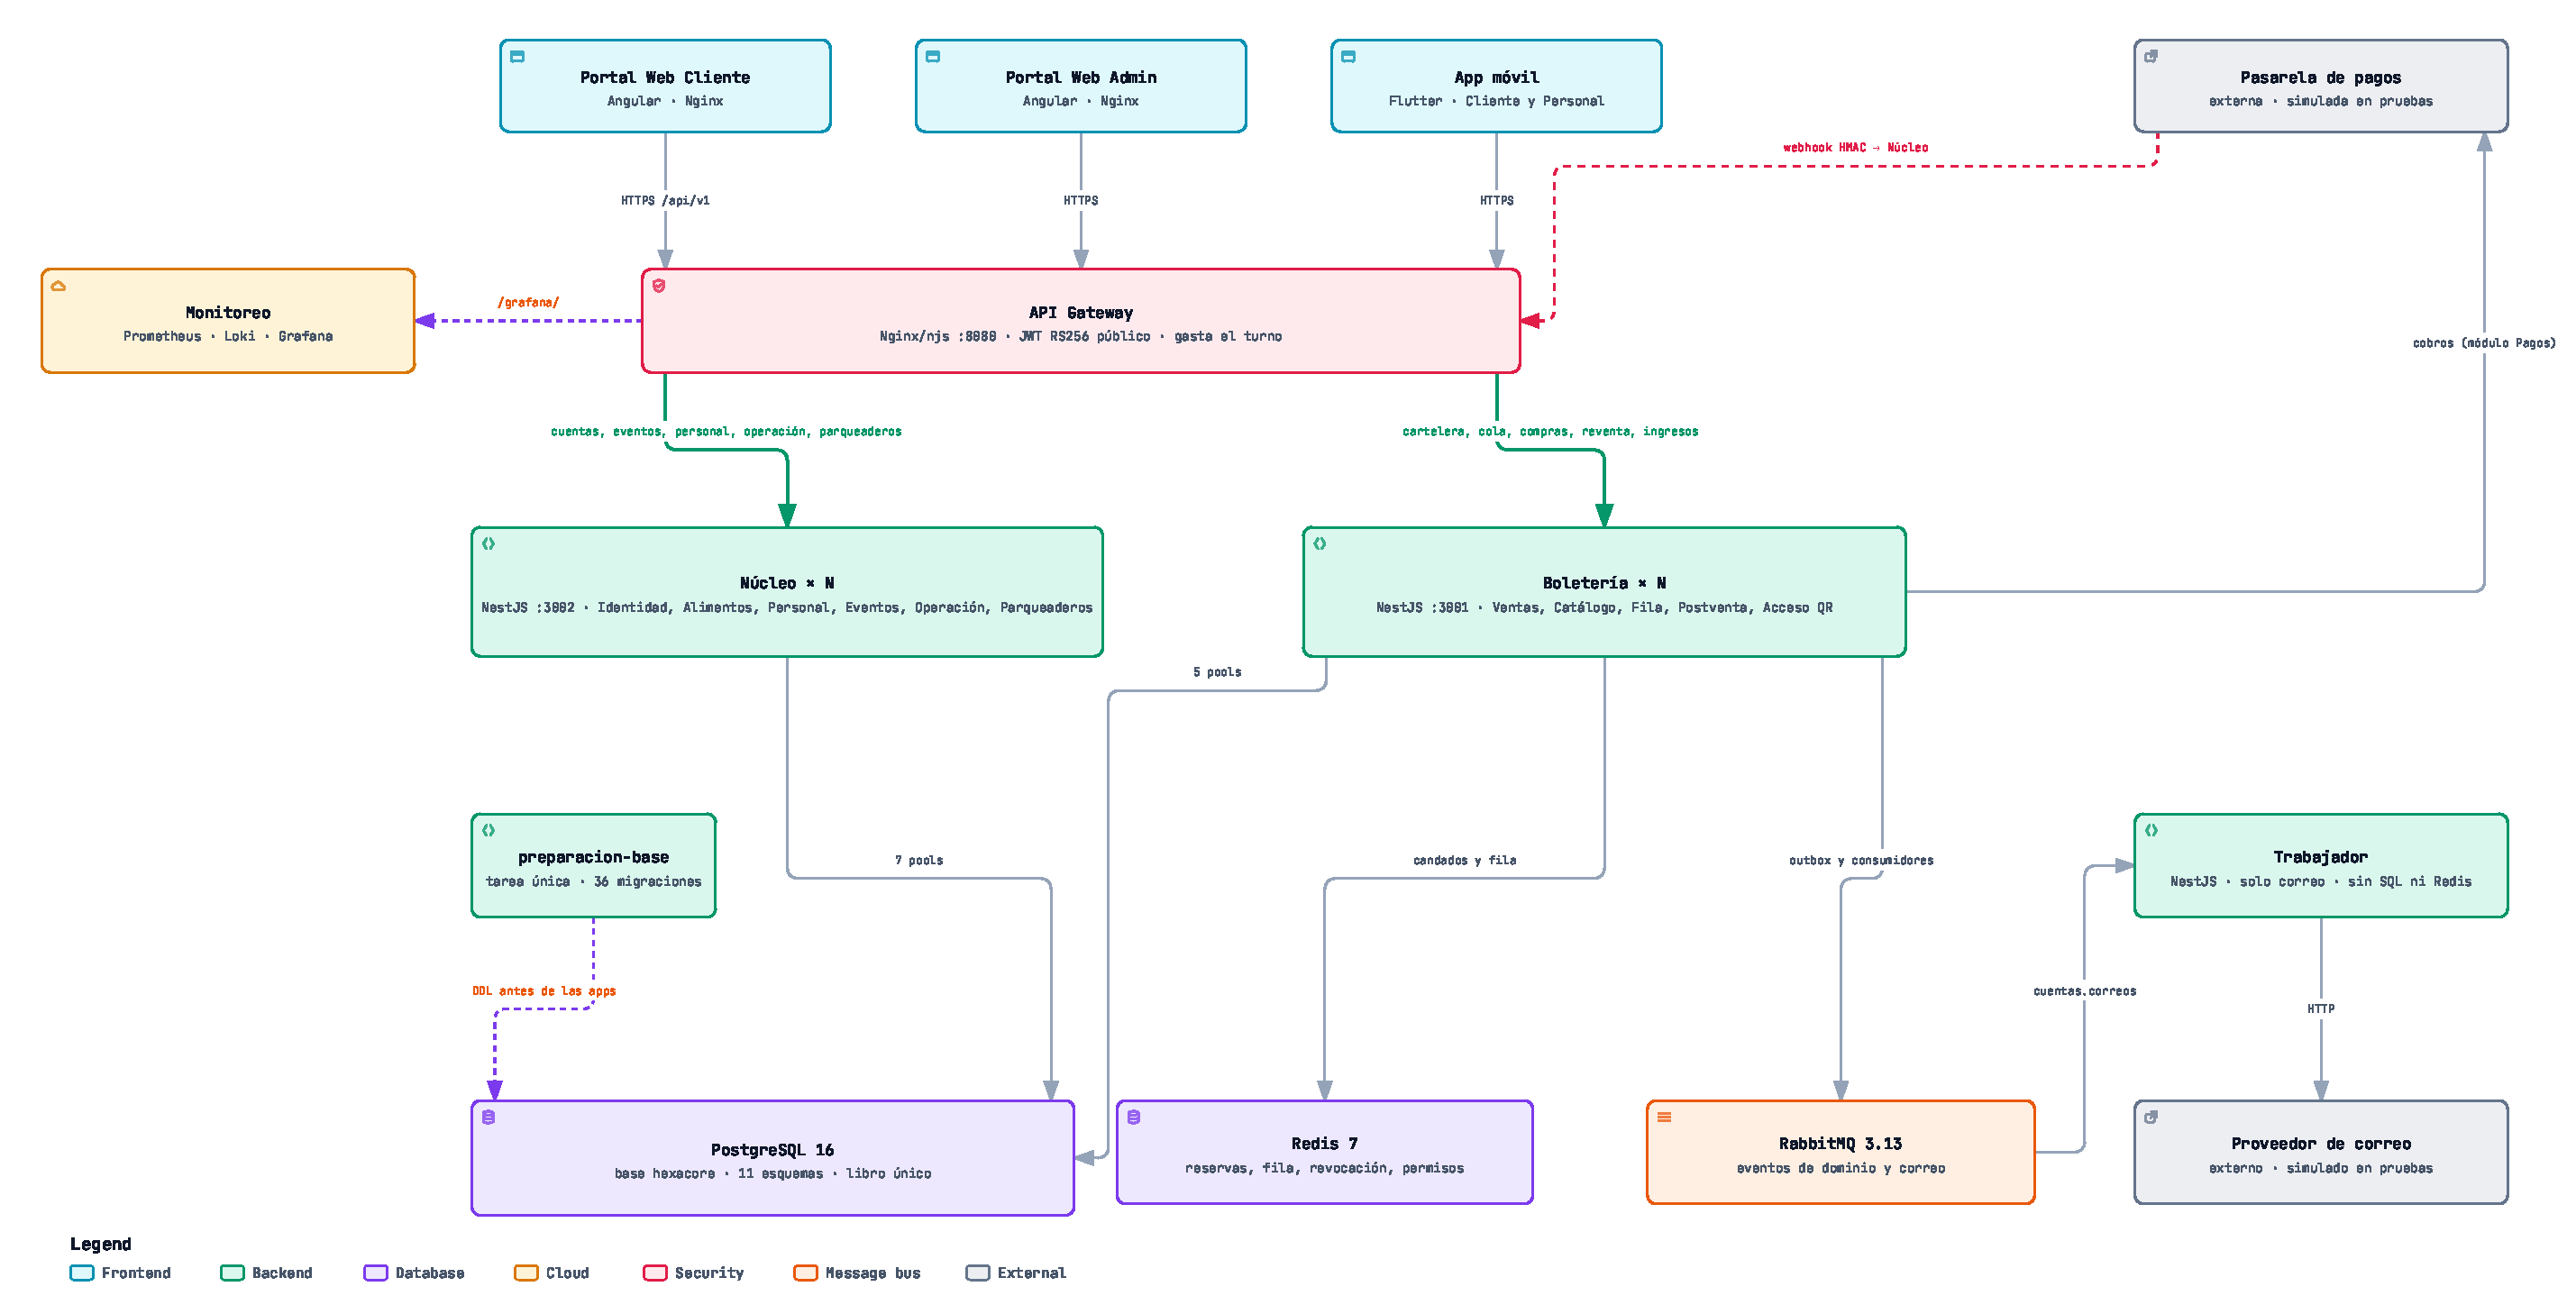
\includegraphics[width=\linewidth,height=0.6\textheight,keepaspectratio]{Diagrams/ArchifyPDF/02-contenedores.pdf}
\end{columns}
\nota{Antes: 14 servicios propuestos. Ahora: Núcleo, Boletería y Trabajador detrás del gateway.}
\end{frame}

\begin{frame}{Antes: contenedores propuestos en ADR-14/15}
\centering
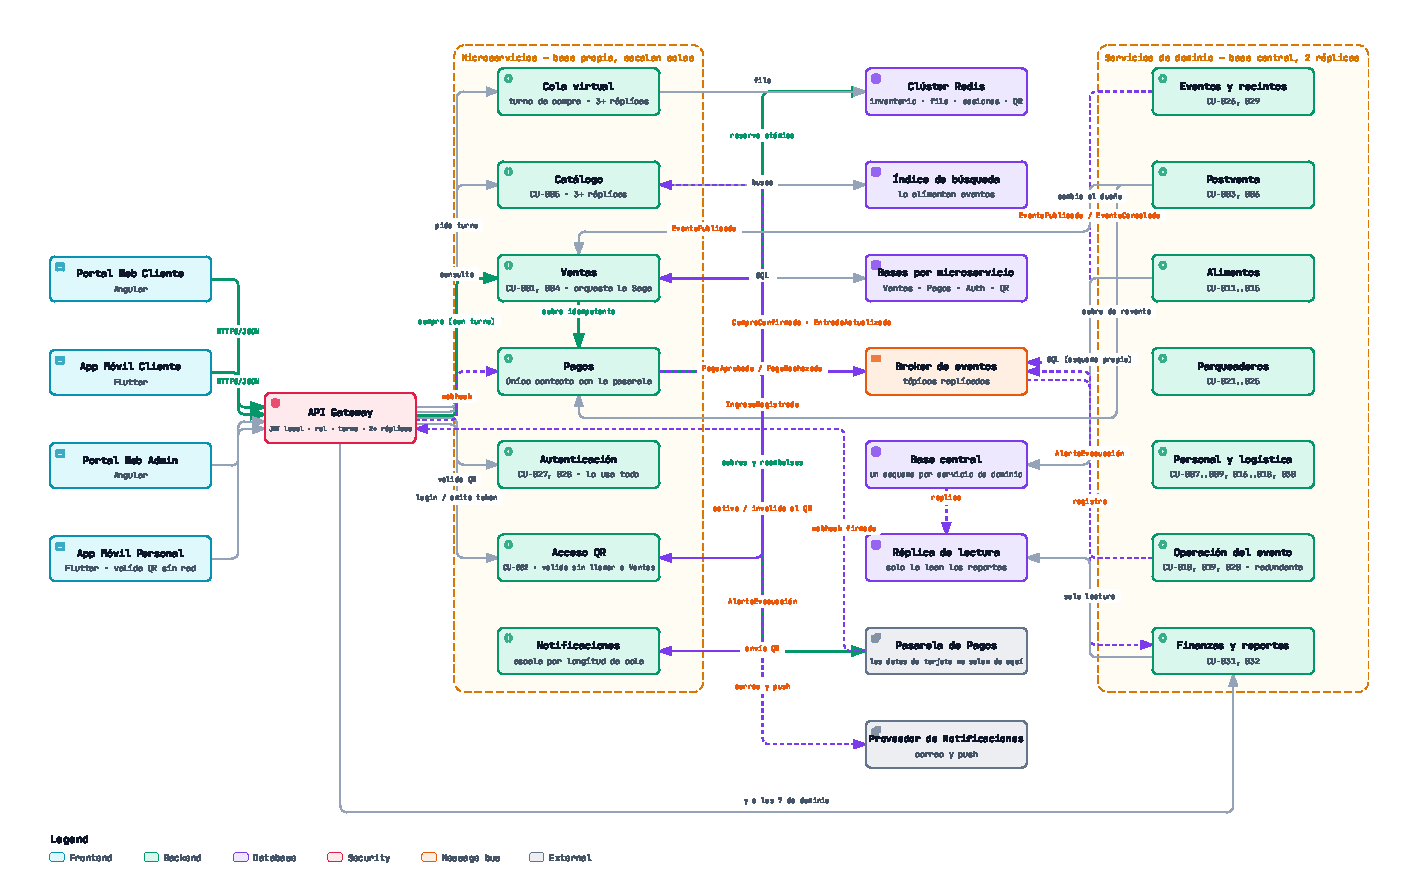
\includegraphics[width=\textwidth,height=0.78\textheight,keepaspectratio]{Historico/Contenedores-ADR14-15.pdf}
\end{frame}

\begin{frame}{Ahora: contenedores vigentes}
\centering
\HexContenedores
\end{frame}

\begin{frame}{Qué cambió, pieza por pieza}
\footnotesize
\begin{tabular}{@{}L{2.6cm}L{4.6cm}L{6.0cm}@{}}
\toprule
& \textbf{Antes (ADR-14/15)} & \textbf{Ahora (ADR-16)}\\
\midrule
Programas & 14 servicios propuestos & \textbf{Núcleo} (7 módulos), \textbf{Boletería} (entradas) y \textbf{Trabajador} (correo)\\[0.3em]
Datos & Una base por dominio (8 bases) & Un PostgreSQL con \cifra{11 esquemas} y 36 migraciones, uno por módulo\\[0.3em]
Entrada & API Gateway & El mismo gateway: JWT RS256, rol y turno de la cola virtual\\[0.3em]
Comunicación & HTTP y RabbitMQ & HTTP por el gateway; eventos por RabbitMQ con bandeja de salida\\[0.3em]
Permisos & En el token & Roles y permisos vigentes en Redis (CU-028), sin volver a iniciar sesión\\[0.3em]
Escalado & Por servicio & Réplicas de Núcleo y Boletería; el gateway las descubre por DNS\\[0.3em]
Operación & --- & Prometheus, Loki y Grafana tras el gateway; imágenes en GHCR y CD\\
\bottomrule
\end{tabular}
\end{frame}

\begin{frame}{Decisiones y concesiones}
\begin{itemize}\setlength\itemsep{0.4em}
\item \textbf{Pagos es un módulo}, no un servicio: el Núcleo y Boletería cobran con la misma API
local, y el webhook de la pasarela llega al Núcleo.
\item \textbf{Las migraciones se aplican una vez, antes de arrancar}: una tarea
(\texttt{preparacion-base}) las corre; las réplicas no migran al arrancar.
\item \textbf{Compartir la base no hace atómico todo}: entre módulos siguen las proyecciones y la
bandeja de salida, con consistencia eventual.
\item \textbf{Concesión aceptada:} menos coordinación entre programas, a cambio de un punto de
fallo SQL y un despliegue compartido.
\end{itemize}
\nota{\codigo{App/backend/apps/nucleo/nucleo.module.ts}{NucleoModule} · \codigo{App/backend/compartido/persistencia/historia.ts}{Migraciones vigentes}}
\end{frame}

\begin{frame}{Despliegue vigente}
\centering
\HexDespliegue
\end{frame}

% =============================================================================
\section{Demostración del prototipo}
% =============================================================================

\begin{frame}{Guion de diez minutos}
\footnotesize
\begin{tabular}{@{}L{2.0cm}L{4.6cm}L{5.6cm}r@{}}
\toprule
\textbf{Integrante} & \textbf{Casos de uso} & \textbf{Qué se muestra} & \textbf{min}\\
\midrule
Daniel & CU-001--005, CU-021--023 & Cartelera, compra con turno y pago; QR de la entrada; reserva e ingreso al parqueadero & 2,5\\[0.3em]
Samuel & CU-006--010, CU-024--026, CU-028 & Reventa; personal, turnos y asistencia; evacuación; cobro y ocupación del parqueadero; eventos; roles y permisos & 2,5\\[0.3em]
Sebastián & CU-011--015, CU-027--029 & Pedidos de alimentos, menú, preparación y entrega; cuentas; recintos y zonas & 2,5\\[0.3em]
Diego & CU-016--020, CU-030--032 & Logística, asignación y turnos del personal; monitoreo del evento; proveedores y pagos & 2,5\\
\bottomrule
\end{tabular}

\vspace{0.6em}
Cada integrante muestra sus casos de uso; los recorridos automáticos con Playwright sirven para
mostrar varios casos en poco tiempo.
\nota{Reparto formal de casos de uso del SRS (anexo).}
\end{frame}

\begin{frame}[fragile]{Cómo se corre en vivo}
\small
\begin{itemize}\setlength\itemsep{0.4em}
\item \textbf{Sistema:} \texttt{cd App/infra \&\& ./iniciar.sh -{}-datos-demo -{}-monitoreo}
\item \textbf{Casos de Samuel} (pantallas de 1,5 s, unos 1,5 min):\\
\texttt{cd App/frontend/demo-playwright \&\& npm run demo:ver -{}- casos/05 casos/07 casos/08}\\
(evacuación CU-010, reventa CU-006 y roles CU-028)
\item \textbf{Casos de Sebastián:} \texttt{npm -{}-prefix App/e2e run demo -{}- cu015}
\item \textbf{Plan B:} los videos que deja \texttt{npm run demo:informe}, por si la red o el
portátil fallan.
\end{itemize}
\nota{Guías: App/frontend/demo-playwright/GUIA-DEMOSTRACION.md y App/e2e/README.md.}
\end{frame}

% =============================================================================
\section{Asignación de atributos de calidad}
% =============================================================================

\begin{frame}{Quién responde por cada atributo}
\scriptsize
\begin{tabular}{@{}L{3.6cm}L{2.0cm}L{2.3cm}L{5.4cm}@{}}
\toprule
\textbf{Atributo} & \textbf{Responsable} & \textbf{RNF del SAD} & \textbf{Demostración en vivo}\\
\midrule
Desempeño (carga) & Samuel & RNF-07, 08, 10 & Prueba de carga y su reporte interpretado\\
Disponibilidad (resiliencia) & Samuel & RNF-03, 04, 09, 17 & Réplicas, caída y recuperación; tres computadores\\
Monitoreo y logs & Samuel & RNF-19 & Tablero de CPU, memoria y logs por el gateway\\
\midrule
Seguridad (OWASP) & Sebastián & RNF-05, 06 & ZAP en Actions: cero High\\
Safety (transacciones) & Sebastián & RNF-01, 02, 11 & Código que verifica las transacciones con dinero\\
Modificabilidad & Sebastián & RNF-13 & Parámetros sin recompilar\\
\midrule
Desplegabilidad & Diego & RNF-15 & Merge a \texttt{main} y despliegue sin clics\\
Comprobabilidad & Diego & RNF-18 & Reporte de cobertura en GitHub Actions\\
\midrule
Integrabilidad (pagos) & Daniel & RNF-16 & Protocolos y pago con la pasarela, en detalle\\
Usabilidad (arq. de información) & Daniel; todos aportan & RNF-12, 14 & Patrón de cada grupo de pantallas\\
\bottomrule
\end{tabular}
\nota{Los 19 RNF del SAD quedan cubiertos. Detalle: Documentation/Work/DISTRIBUCION-ATRIBUTOS.md.}
\end{frame}

% =============================================================================
\section{Diseño e implementación de los atributos}
% =============================================================================

% --- Samuel: desempeño, disponibilidad y monitoreo ---------------------------
% Diapositivas de los atributos de calidad de Samuel Emperador: desempeño,
% disponibilidad y monitoreo y logs. Las incluye Presentacion.tex con \input.
% Las cifras son las de App/infra/informe-atributos/ (12/11/2026) y el detalle,
% en el SAD, sección «Atributos de calidad sobre la arquitectura vigente».
% Ocupan el tramo 16:00--22:00 del guion; el diagrama de despliegue está en los anexos.

% ---------------------------------------------------------------------------
\begin{frame}{Tres atributos, una misma evidencia}
\small
\begin{tabular}{L{2.4cm}L{5.2cm}L{5.5cm}}
\toprule
\textbf{Atributo} & \textbf{Lo que se pide} & \textbf{Cómo se demuestra}\\
\midrule
Desempeño & Prueba de carga en el momento, con reporte e interpretación &
\texttt{prueba-carga.py}: 3 casos de uso, 5 niveles, CPU por contenedor\\[0.3em]
Disponibilidad & Balanceo entre réplicas; tumbar una y que el sistema siga y se recupere &
\texttt{demo-disponibilidad.sh}: \texttt{kill -9} con tráfico en curso\\[0.3em]
Monitoreo y logs & CPU y memoria por instancia y logs desde el mismo punto de entrada &
Grafana en \texttt{/grafana/}, servido por el API Gateway\\
\bottomrule
\end{tabular}

\vspace{0.8em}
\begin{block}{Una sola orden}
\texttt{./iniciar.sh -{}-monitoreo} levanta el sistema y el tablero. El monitoreo es la evidencia
visual de los otros dos: mientras corre la carga se ve subir la CPU, y al tumbar una réplica se ve
caer y volver.
\end{block}
\franja{16:00--16:30 · Samuel · Desempeño RNF-07/08/10, Disponibilidad RNF-03/04/09/17, Monitoreo RNF-19.}
\end{frame}

% ---------------------------------------------------------------------------
\begin{frame}{Desempeño · diseño}
\small
\begin{columns}[T]
\begin{column}{0.47\textwidth}
\textbf{Escenario de calidad}\\[0.3em]
\begin{tabular}{@{}L{1.7cm}L{4.6cm}@{}}
Fuente & Clientes y organizadores en la apertura\\
Estímulo & Hasta 200 usuarios pidiendo sin pausa\\
Artefacto & Boletería (CU-006) y Núcleo (CU-025, CU-026)\\
Entorno & 1 réplica y luego 2 del Núcleo\\
Respuesta & Atender sin errores; crecer al replicar\\
Medida & \leavevmode\cifra{p95 $\leq$ 500 ms} y 0 fallos hasta 200 usuarios; $\geq$ 1,7$\times$ al duplicar\\
\end{tabular}
\end{column}
\begin{column}{0.5\textwidth}
\textbf{Tácticas}\\[0.3em]
\begin{itemize}\setlength\itemsep{0.3em}
\item \textbf{Introducir concurrencia:} réplicas de Núcleo y Boletería; cada una, un proceso Node
con su núcleo.
\item \textbf{Balancear:} nginx reparte por turnos y descubre réplicas en el DNS de Docker cada 5 s.
\item \textbf{Acotar la demanda:} pool de 10 conexiones y espera máxima de 3 s por programa.
\item \textbf{Reducir la sobrecarga:} el token se verifica en local; nadie le pregunta a Identidad
en cada petición.
\end{itemize}
\end{column}
\end{columns}
\franja{16:30--17:30 · Samuel · Ensayo local; RNF-07 fija 2\,000 usuarios sobre CU-001 y RNF-10 habla de Entradas.}
\end{frame}

% ---------------------------------------------------------------------------
\begin{frame}{Desempeño · resultados con una réplica}
\begin{columns}[T]
\begin{column}{0.6\textwidth}
\begin{tikzpicture}
\begin{axis}[width=\linewidth, height=4.6cm, xlabel={Usuarios simultáneos}, ylabel={p95 (ms)},
  xmode=log, log basis x=10, xtick={1,10,50,100,200}, xticklabels={1,10,50,100,200},
  ymin=0, ymax=560, legend style={font=\scriptsize, draw=none, fill=none, at={(0.5,-0.3)}, anchor=north, legend columns=2},
  tick label style={font=\scriptsize}, label style={font=\small}, grid=major, grid style={gray!20}]
\addplot[hexaacento, thick, mark=*] coordinates {(1,4.5)(10,13.5)(50,38.4)(100,84.9)(200,150.3)};
\addplot[hexazul, thick, mark=square*] coordinates {(1,4.9)(10,16.4)(50,84.8)(100,168.0)(200,355.0)};
\addplot[hexaparcial, thick, mark=triangle*] coordinates {(1,5.3)(10,21.0)(50,93.3)(100,203.7)(200,310.6)};
\addplot[hexapend, dashed, domain=1:200] {500};
\legend{CU-006 reventa, CU-026 eventos, CU-025 parqueadero, umbral RNF-07}
\end{axis}
\end{tikzpicture}
\end{column}
\begin{column}{0.38\textwidth}
\small
\begin{tabular}{@{}lrr@{}}
\toprule
& \textbf{p95, 200 us.} & \textbf{Máx. pet/s}\\
\midrule
CU-006 & 150 ms & 1\,906\\
CU-026 & 355 ms & 760\\
CU-025 & 311 ms & 759\\
\bottomrule
\end{tabular}

\vspace{0.8em}
\cifra{0 fallos} en más de 100\,000 peticiones, todas por el gateway.

\vspace{0.5em}
Los tres quedan en \cifra{p95 $\leq$ 500 ms} en todos los niveles medidos, hasta 200 usuarios.
\end{column}
\end{columns}
\franja{17:30--18:15 · Samuel · Informe: App/infra/informe-atributos/CARGA-1-replica.md.}
\end{frame}

% ---------------------------------------------------------------------------
\begin{frame}{Desempeño · interpretación}
\begin{columns}[T]
\begin{column}{0.52\textwidth}
\begin{tikzpicture}
\begin{axis}[width=\linewidth, height=4.6cm, xlabel={Usuarios simultáneos}, ylabel={Peticiones/s},
  xmode=log, log basis x=10, xtick={1,10,50,100,200}, xticklabels={1,10,50,100,200},
  ymin=0, ymax=1500, legend style={font=\scriptsize, draw=none, fill=none, at={(0.5,-0.3)}, anchor=north, legend columns=2},
  tick label style={font=\scriptsize}, label style={font=\small}, grid=major, grid style={gray!20}]
\addplot[hexaparcial, thick, mark=triangle*] coordinates {(1,266)(10,746)(50,750)(100,673)(200,759)};
\addplot[hexaparcial, thick, dashed, mark=triangle] coordinates {(1,193)(10,934)(50,1052)(100,1275)(200,1385)};
\addplot[hexazul, thick, mark=square*] coordinates {(1,315)(10,760)(50,715)(100,683)(200,675)};
\addplot[hexazul, thick, dashed, mark=square] coordinates {(1,245)(10,1030)(50,1196)(100,1123)(200,1106)};
\legend{CU-025 · 1 réplica, CU-025 · 2 réplicas, CU-026 · 1 réplica, CU-026 · 2 réplicas}
\end{axis}
\end{tikzpicture}
\end{column}
\begin{column}{0.46\textwidth}
\small
\begin{itemize}\setlength\itemsep{0.35em}
\item \textbf{El rendimiento se topa:} desde ahí, más usuarios es solo más espera. Ley de Little:
usuarios = rendimiento $\times$ tiempo de respuesta.
\item \textbf{Cuello de botella: el proceso Node}, en \cifra{101--106\,\%} de un núcleo. Ejecuta la
aplicación en un solo hilo.
\item \textbf{Por eso replicar funciona:} con 2 réplicas, CU-025 \cifra{+82\,\%} (1,82$\times$) y
CU-026 \cifra{+57\,\%}.
\item \textbf{Siguiente límite:} PostgreSQL en 325\,\% con 2 réplicas en CU-025. Todavía reparte el
trabajo en varios núcleos.
\end{itemize}
\end{column}
\end{columns}
\franja{18:15--19:00 · Samuel · Se escaló el Núcleo; el escalado de Boletería (Entradas) sigue sin medir.}
\end{frame}

% ---------------------------------------------------------------------------
\begin{frame}{Disponibilidad · diseño}
\footnotesize
\begin{columns}[T]
\begin{column}{0.47\textwidth}
\textbf{Escenario de calidad}\\[0.3em]
\begin{tabular}{@{}L{1.7cm}L{4.6cm}@{}}
Fuente & Falla interna: muere un proceso\\
Estímulo & \texttt{kill -9} a una réplica con tráfico en curso\\
Artefacto & Réplicas de Boletería y Núcleo, gateway, Docker\\
Entorno & Operación normal con carga constante\\
Respuesta & Las demás absorben el tráfico; la caída se recupera sola\\
Medida & \leavevmode\cifra{0 fallos}; recuperación \cifra{$\leq$ 30 s} sin intervención (RNF-04)\\
\end{tabular}
\end{column}
\begin{column}{0.5\textwidth}
\textbf{Tácticas}\\[0.3em]
\begin{itemize}\setlength\itemsep{0.3em}
\item \textbf{Redundancia activa:} varias réplicas sin estado en memoria; comparten PostgreSQL y Redis.
\item \textbf{Reintento de lecturas:} si una réplica falla antes de responder, nginx lleva la lectura a
otra. Las escrituras no se reintentan.
\item \textbf{Detección:} sonda de salud cada 10 s en Docker; el gateway detecta errores y tiempos
agotados al enviar tráfico.
\item \textbf{Reintroducción:} \texttt{restart: unless-stopped}; el DNS de Docker vuelve a publicar
la réplica.
\item \textbf{Réplicas seguras:} los trabajos de fondo toman sus filas con \texttt{SKIP LOCKED}; dos
réplicas no procesan la misma a la vez.
\end{itemize}
\end{column}
\end{columns}
\franja{19:00--19:45 · Samuel · Escenario: caída de un proceso. No cubre apagar un computador ni la caída de PostgreSQL.}
\end{frame}

% ---------------------------------------------------------------------------
\begin{frame}{Disponibilidad · resultados}
\begin{columns}[T]
\begin{column}{0.55\textwidth}
\small
\begin{tabular}{@{}L{3.6cm}L{1.8cm}L{1.6cm}@{}}
\toprule
& \textbf{Boletería ×3} & \textbf{Núcleo ×2}\\
\midrule
Reparto de 30 peticiones & 10 / 10 / 10 & 15 / 15\\
Peticiones en los 8 s tras el \texttt{kill -9} & \leavevmode\cifra{484} & \leavevmode\cifra{509}\\
Fallidas & \leavevmode\cifra{0} & \leavevmode\cifra{0}\\
Reintentadas en otra réplica & 1 & 1\\
Docker la reinicia y está sana & \leavevmode\cifra{8--13 s} & \leavevmode\cifra{8 s}\\
Vuelve al reparto & Sí & Sí\\
\bottomrule
\end{tabular}
\end{column}
\begin{column}{0.43\textwidth}
\small
\begin{itemize}\setlength\itemsep{0.35em}
\item \textbf{Ninguna lectura falló:} la que la réplica no alcanzó a responder se reintentó en otra.
\item \textbf{Dentro de RNF-04:} 8--13 s frente a los 30 s permitidos. No mide el 99,9\,\% mensual.
\item \textbf{El Núcleo también se replica:} la demo de los 8 casos de uso pasa contra 2 réplicas.
\item \textbf{Límites:} un \texttt{POST} en curso no se reintenta (no se duplica una escritura);
PostgreSQL, Redis y RabbitMQ siguen siendo una instancia.
\end{itemize}
\end{column}
\end{columns}
\franja{19:45--20:30 · Samuel · Informe: App/infra/DEMOSTRACION-ATRIBUTOS.md, sección 3.}
\end{frame}

% ---------------------------------------------------------------------------
\begin{frame}{Monitoreo y logs · diseño}
\begin{columns}[T]
\begin{column}{0.56\textwidth}
\centering
\begin{tikzpicture}[font=\scriptsize, node distance=0.45cm and 0.45cm,
  caja/.style={draw=hexazul, fill=hexagris, rounded corners=2pt, align=center, minimum width=2.1cm, minimum height=0.7cm},
  flecha/.style={-{Stealth[length=2mm]}, thick, hexaacento}]
\node[caja] (docker) {Contenedores\\(API de Docker)};
\node[caja, right=of docker] (exp) {Exportador\\CPU y memoria};
\node[caja, below=of exp] (prom) {Prometheus\\muestra cada 2 s};
\node[caja, below=of docker] (salida) {Salida de los\\contenedores};
\node[caja, below=of salida] (promtail) {Promtail};
\node[caja, right=of promtail] (loki) {Loki};
\node[caja, fill=hexaacento!20, right=0.8cm of prom] (graf) {Grafana\\7 paneles};
\node[caja, fill=hexazul!15, above=of graf] (gw) {API Gateway\\\texttt{/grafana/}};
\draw[flecha] (docker) -- (exp);
\draw[flecha] (exp) -- (prom);
\draw[flecha] (salida) -- (promtail);
\draw[flecha] (promtail) -- (loki);
\draw[flecha] (prom) -- (graf);
\draw[flecha] (loki) -| (graf);
\draw[flecha] (gw) -- (graf);
\end{tikzpicture}
\end{column}
\begin{column}{0.42\textwidth}
\small
\textbf{Paneles:} instancias vivas · CPU por instancia · memoria por instancia · peticiones por
réplica · respuestas por código · latencia p95 · logs filtrables por servicio.

\vspace{0.6em}
\textbf{Sin instrumentar los programas:} las métricas salen de Docker y el tráfico del log del
gateway (\texttt{upstream=}, \texttt{rt=}).

\vspace{0.6em}
\textbf{Por qué no cAdvisor:} en Docker Desktop (containerd) las versiones 0.49 y 0.52 no ven los
contenedores. El exportador publica las mismas métricas: en Linux se vuelve a cAdvisor sin tocar
el tablero.
\end{column}
\end{columns}
\franja{20:30--21:15 · Samuel · Despliegue con réplicas y monitoreo: anexo «despliegue».}
\end{frame}

% ---------------------------------------------------------------------------
\begin{frame}{Demostración en vivo · unos 6,5 minutos}
\footnotesize
\begin{tabular}{@{}cL{5.3cm}L{5.0cm}r@{}}
\toprule
\# & \textbf{Qué se corre} & \textbf{Qué se señala} & \textbf{Tiempo}\\
\midrule
1 & Abrir \texttt{localhost:8080/grafana/} & Instancias vivas, CPU, memoria y logs & 30 s\\
2 & \texttt{./prueba-carga.py -{}-rapida} & La tabla por nivel y la CPU subiendo en Grafana & 2 min\\
3 & Leer la interpretación impresa & Dónde se satura cada caso de uso y por qué & 1 min\\
4 & \texttt{./demo-disponibilidad.sh} & Reparto, réplica caída, 0 fallos, recuperación & 1,5 min\\
5 & \texttt{SERVICIO=nucleo ./demo-disponibilidad.sh -{}-seguido} & Lo mismo con el Núcleo & 40 s\\
6 & \texttt{./demo-disponibilidad.sh -{}-restaurar} & Todo vuelve a una réplica & 10 s\\
\bottomrule
\end{tabular}

\vspace{0.5em}
Todo desde \texttt{App/infra}. Guion completo en \texttt{App/infra/DEMOSTRACION-ATRIBUTOS.md}.
\franja{Se ejecuta en el bloque de demostraciones (34:00--44:00), que hoy le asigna 150 s: tiempo por acordar.}
\end{frame}

% ---------------------------------------------------------------------------
\begin{frame}{Límites medidos y siguiente paso}
\footnotesize
\begin{columns}[T]
\begin{column}{0.5\textwidth}
\textbf{Lo que no se cumple o no se midió}
\begin{itemize}\setlength\itemsep{0.2em}
\item \textbf{RNF-07:} medido hasta 200 usuarios y sobre CU-006/025/026; fija 2\,000 sobre CU-001.
En un solo portátil el generador compite por la CPU con lo que mide.
\item \textbf{RNF-10:} con 2 Núcleos, CU-025 llega a \cifra{1,82$\times$} y CU-026 a \cifra{1,57$\times$}
(pide 1,7$\times$ en Entradas, que no se midió).
\item \textbf{RNF-08, RNF-09 y RNF-17:} asignados, aún sin medición.
\item \textbf{Monitoreo:} sin alertas automáticas, 2 días de retención y un solo nodo.
\item Todo compartía 11 núcleos; el p95 varía ±30\,\% entre corridas.
\end{itemize}
\end{column}
\begin{column}{0.48\textwidth}
\textbf{Qué se haría después}
\begin{itemize}\setlength\itemsep{0.2em}
\item Más réplicas de Núcleo y Boletería, hasta que PostgreSQL o el gateway sean el límite.
\item Guardar unos segundos en Redis el panel de CU-025, la lectura más cara.
\item Alertas en Grafana sobre instancias caídas y p95.
\item Repetir la carga con el generador en otra máquina.
\end{itemize}
\end{column}
\end{columns}
\franja{21:15--22:00 · Samuel · Implementado $\neq$ comprobado; comprobado en un ensayo $\neq$ RNF completo.}
\end{frame}


% --- Sebastián: seguridad, Safety y modificabilidad --------------------------
\begin{frame}{Seguridad · diseño y ubicación de controles}
\begin{itemize}\setlength\itemsep{0.3em}
\item \textbf{RNF-05/06.} JWT RS256: la llave privada solo en Identidad (Núcleo); la pública en el gateway y en Boletería.
\item \textbf{El gateway} valida el JWT y el rol; los módulos con permisos dinámicos deciden con los permisos vigentes.
\item \textbf{Los servicios} aplican rol, propiedad del recurso, estado y autoridad administrativa vigente.
\item \textbf{Redis} comparte revocación y roles; un dato ilegible responde 503, sin recuperar privilegios viejos.
\item \textbf{Los paneles en vivo (SSE)} revalidan sesión y permiso y cierran con un mensaje saneado.
\end{itemize}
\nota{Sebastián · \codigo{App/gateway/autenticacion.js}{Gateway} · \codigo{App/backend/compartido/seguridad/sesion-valida.guard.ts}{Guarda común} · \codigo{App/shared/seguridad/permisos.md}{Contrato}}
\end{frame}

\begin{frame}{Seguridad · evidencia y escaneo OWASP}
\small
\begin{itemize}\setlength\itemsep{0.25em}
\item \cifra{167/167} protegidas de 186 declaradas/181 expuestas: evidencia histórica por gateway y backend directo; combinaciones publicadas, no cobertura universal.
\item ZAP reutilizado \textbf{después de desplegar}: dos portales y GET públicos/perfil Cliente autenticado. HTML/JSON saneados con todas las alertas.
\item CI111: ZAP 2.17.0, \cifra{0 High}, 10 Medium y 4 Informational conservadas; sin categoría Critical. npm: producción/Critical cero, 20 moderadas de desarrollo backend.
\item \textbf{Alcance:} runner temporal aprobado. Samuel confirma que el servidor de presentación nunca se creó; faltan nombres controlados por el equipo y conexión de Diego.
\item RNF-05/06 parciales: ZAP pasivo no ejecuta JS ni sustituye pruebas de autorización/PAN.
\end{itemize}
\nota{Demo: \href{https://github.com/Emperador24/HEXACORE/actions/runs/44000569216}{Actions CI111} $\rightarrow$ trabajo OWASP $\rightarrow$ Summary/Artifacts $\rightarrow$ \texttt{atributos-sebastian} $\rightarrow$ \path{owasp.html} / \path{owasp.json}. Ejecución completada: 20 GET, 1 autenticado. No se repite por este cambio documental.}
\end{frame}

\begin{frame}{Safety · transacciones con dinero}
\small
\begin{itemize}\setlength\itemsep{0.3em}
\item \textbf{Durante:} bloqueos, reservas, unicidad, idempotencia y estados. Después: nuevo verificador identificado \texttt{REPEATABLE READ READ ONLY}.
\item Cruza negocio/libro: importe exacto, moneda, referencia, clave, resultado, actor/tiempo e historial. No llama proveedores ni escribe/compensa.
\item \textbf{Demo:} original consistente (0), doble con un centavo distinto (1), original conservado (0). Pendiente/incierto/parcial (2); configuración inválida (3).
\item RNF-01: histórico 50 compradores reutilizado; ocho checkouts actuales no sustituyen ese umbral. RNF-02: proyección QR asíncrona, prueba espera convergencia.
\item RNF-11 parcial: política de un año sin antigüedad acreditada; actor del negocio enlazado al dominio solicitante del libro. SQL no es no repudio criptográfico.
\item F12 detectado, sin resolver. Libro de reembolso sin referencia original persistida: se informa parcial.
\end{itemize}
\nota{Sebastián · herramientas/verificar-transaccion.cjs y test/safety/demostrar.cjs; solo fixtures con proveedores simulados.}
\end{frame}

\begin{frame}{Modificabilidad · configuración sin recompilar}
\small
\begin{tabular}{@{}L{3.7cm}L{5.4cm}L{3.4cm}@{}}
\toprule Parámetro & Efecto que se comprueba & Rechazo\\\midrule
\texttt{PUERTO} & 3002 a 3003: HTTP, gateway y sonda; recrear solo aplicaciones necesarias & Puerto 0\\[0.4em]
\texttt{configuracion.js}: API & Petición real de Chromium: API por defecto a \texttt{/ensayo-api/v1} & URL inválida\\[0.4em]
Espera máxima PostgreSQL & 3000 a 1000 ms: consulta de 4 s cancelada por DataSource compilado & 499 ms\\
\bottomrule
\end{tabular}
\par\medskip
Image IDs SHA-256 iguales antes/después; \texttt{--no-build}. Sin recarga en caliente.
\textbf{Tácticas:} cohesión de responsabilidades, contratos/intermediarios y restricción de dependencias; enlace al arranque.
\nota{RNF-13 parcial: PR 60, regla «Acceso general», solo Monitoreo y pruebas; contrato sin ampliar. ADR-16 conserva despliegues coordinados.}
\end{frame}

% --- Diego: desplegabilidad y comprobabilidad --------------------------------
\begin{frame}{Desplegabilidad · del merge a producción sin clics}
\small
\begin{enumerate}\setlength\itemsep{0.3em}
\item Merge a \texttt{main}: GitHub Actions corre el CI (8 trabajos).
\item El CD compila las 8 imágenes para amd64 y arm64 y las publica en GHCR por digest.
\item «Desplegar en producción» entra por SSH al servidor y corre \texttt{desplegar.sh sha-<commit>}.
\item Si la versión nueva no queda sana, vuelve sola a la anterior (RNF-15: reversión).
\end{enumerate}
\textbf{Para la demo:} el paso de despliegue solo corre cuando existe el servidor
(\texttt{PRODUCCION\_DOMINIO}); hoy sale omitido. Falta crear la máquina y sus secretos.
\nota{Diego · \codigo{.github/workflows/cd.yml}{cd.yml} · \codigo{App/infra/desplegar.sh}{desplegar.sh}}
\end{frame}

\begin{frame}{Comprobabilidad · pruebas y cobertura}
\begin{itemize}\setlength\itemsep{0.35em}
\item \textbf{RNF-18:} cada servicio se prueba sin levantar los demás; base, broker, pasarela y correo se reemplazan por dobles.
\item \textbf{En el CI:} \cifra{1\,141 pruebas unitarias}, pruebas HTTP contra el Núcleo, Boletería y el Trabajador reales, portales, app móvil y gateway.
\item \textbf{Cobertura:} \texttt{npm run test:cov:total} une las unitarias y las e2e por línea; los módulos de Samuel están al 100\,\%.
\item \textbf{Falta:} publicar el reporte de cobertura de todos los servicios como paso de GitHub Actions.
\end{itemize}
\nota{Diego · \codigo{.github/workflows/ci.yml}{ci.yml} · \codigo{App/backend/test/cobertura-total.cjs}{cobertura-total.cjs}}
\end{frame}

% --- Daniel: integrabilidad y usabilidad --------------------------------------
\begin{frame}{Integrabilidad · cómo se conecta el sistema}
\small
\begin{columns}[T]
\begin{column}{0.48\textwidth}
\textbf{Interno}
\begin{itemize}\setlength\itemsep{0.2em}
\item HTTP por el API Gateway, con JWT.
\item RabbitMQ entre módulos, con bandeja de salida (\texttt{eventos.gestion}, \texttt{ingreso.registrado}).
\item SSE para los paneles en vivo.
\end{itemize}
\end{column}
\begin{column}{0.48\textwidth}
\textbf{Externo: pasarela de pagos}
\begin{itemize}\setlength\itemsep{0.2em}
\item Un módulo Pagos con dos adaptadores: simulado y Stripe (modo de prueba).
\item El proveedor confirma por un webhook firmado que llega al Núcleo.
\item \textbf{RNF-16:} cambiar de pasarela es cambiar el adaptador (\texttt{PAGOS\_PROVEEDOR}), sin tocar Entradas.
\end{itemize}
\end{column}
\end{columns}
\nota{Daniel · \codigo{App/backend/modulos/finanzas/pagos/pasarela-stripe.service.ts}{Adaptador Stripe} · \codigo{App/backend/modulos/finanzas/pagos/pasarela-http.service.ts}{Adaptador HTTP}}
\end{frame}

\begin{frame}{Usabilidad · arquitectura de información}
\footnotesize
\begin{tabular}{@{}L{3.6cm}L{3.0cm}L{6.4cm}@{}}
\toprule
\textbf{Grupo de pantallas} & \textbf{Patrón} & \textbf{Por qué}\\
\midrule
Cartelera (portal cliente) & Matricial & Se filtra por categoría, ciudad, artista y fechas\\
Compra con turno y pago & Secuencial & Pasos fijos: turno, localidad, pago, confirmación\\
Portal administrativo & Jerárquico & Menú por módulo; cada rol ve solo sus módulos (CU-028)\\
App móvil & Jerárquico por rol & Cliente y Personal ven secciones distintas\\
\bottomrule
\end{tabular}

\vspace{0.6em}
\textbf{RNF-12} (5 usuarios nuevos, $\geq$ 80\,\% de éxito) y \textbf{RNF-14} (paridad web y móvil)
siguen sin prueba con usuarios. Cada integrante confirma el patrón de sus pantallas.
\nota{Daniel consolida; todos aportan.}
\end{frame}

% =============================================================================
\section{Cierre}
% =============================================================================

\begin{frame}{Lo que queda abierto}
\small
\begin{itemize}\setlength\itemsep{0.3em}
\item \textbf{RNF-07} se midió hasta 200 usuarios, no 2\,000; \textbf{RNF-10} con Boletería llega a 1,12--1,26$\times$ en un portátil.
\item \textbf{RNF-03} (99,9\,\% mensual) no se mide en una demo: se muestra su mecanismo.
\item \textbf{Seguridad:} escaneo integrado; falta conectar y ejecutar el despliegue de presentación de Diego.
\item \textbf{Desplegabilidad:} servidor de presentación nunca creado; conexión de Diego pendiente, sin dominio del equipo confirmado.
\item \textbf{Comprobabilidad:} falta publicar la cobertura de todos los servicios en Actions.
\item \textbf{Usabilidad:} falta la prueba con cinco usuarios nuevos.
\end{itemize}
\end{frame}

\begin{frame}{Evidencia y entregables}
\begin{itemize}\setlength\itemsep{0.35em}
\item \textbf{SAD actualizado} (\texttt{Documentation/Submission}): arquitectura vigente y diseño de cada atributo.
\item \textbf{Repositorio:} \href{https://github.com/Emperador24/HEXACORE}{github.com/Emperador24/HEXACORE}, rama \texttt{develop}.
\item \textbf{Informes de medición:} \texttt{App/infra/informe-atributos/} (carga, tiempo real, seguridad).
\item \textbf{Reparto de atributos y RNF:} \texttt{Documentation/Work/DISTRIBUCION-ATRIBUTOS.md}.
\end{itemize}
\vspace{1em}
\centering\Large Preguntas
\end{frame}

% =============================================================================
\appendix
\begin{frame}{Anexo: contexto}\centering\HexContexto\end{frame}
\begin{frame}{Anexo: componentes del Núcleo}\centering\HexComponentesNucleo\end{frame}
\begin{frame}{Anexo: componentes de Boletería}\centering\HexComponentesBoleteria\end{frame}
\begin{frame}{Anexo: compra con turno}\centering\HexSecuencia\end{frame}
\begin{frame}{Anexo: reparto formal de casos de uso}
\begin{itemize}
\item Daniel: CU-001--005 y CU-021--023.
\item Samuel: CU-006--010 y CU-024--026; además CU-028 por acuerdo.
\item Sebastián: CU-011--015 y CU-027--029.
\item Diego: CU-016--020 y CU-030--032.
\end{itemize}
\end{frame}

\end{document}
